\documentclass[11pt,a4paper]{article}
\author{TalentSprint}
\date{}
\usepackage{graphicx}
\usepackage{verbatim}
\usepackage{array}
\usepackage{caption}
\usepackage{enumitem}
\usepackage{xcolor}
\usepackage[tikz]{bclogo}
\usepackage{textcomp}
\usepackage{listings}
\usepackage{multicol}
\usepackage{float}
\usepackage{seqsplit} 
\usepackage{setspace}
\usepackage{soul}
\usepackage{latexsym}
\lstset{language=Java,numbers=left, numberstyle=\tiny, numbersep=10pt, showstringspaces=false, breaklines=true,keepspaces=true, columns=flexible}
\usepackage{fancyhdr}
\headheight=14pt
\lhead{\nouppercase{}}
\rhead{\nouppercase{\leftmark}}

\graphicspath{{../Images/}}


\begin{comment}
\setcounter{tocdepth}{1}
\setlength\parindent{0pt}
\parskip=4pt
\def\AnswerBox{\fbox{\begin{minipage}{4in}\hfill\vspace{0.5in}\end {minipage}}}

\thispagestyle{empty}
\vspace{1.5pc}
\topskip0pt
\vspace*{\fill}
\centerline{\sc \Huge Version Control System}
\vspace{2pc}
\vspace*{\fill}
\centerline{Prepared by TalentSprint WISE Team} 
\setcounter{page}{1}
\pagestyle{fancy}
\end{comment}


%========================================================================

% Lengths and widths
\addtolength{\textwidth}{2.5cm}
\addtolength{\hoffset}{0cm}
\setlength{\headsep}{-12pt} % Reduce space between header and content
\setlength{\headheight}{85pt} % If less, LaTeX automatically increases it
\renewcommand{\footrulewidth}{2pt} % Remove footer line
\renewcommand{\headrulewidth}{1pt} % Remove header line
\renewcommand{\seqinsert}{\ifmmode\allowbreak\else\-\fi} % Hyphens in seqsplit
% This two commands together give roughly
% the right line height in the tables
\renewcommand{\arraystretch}{1.3}
\onehalfspacing



% Commands
\newcommand{\SetRowColor}[1]{\noalign{\gdef\RowColorName{#1}}\rowcolor{\RowColorName}} % Shortcut for row colour
\newcommand{\mymulticolumn}[3]{\multicolumn{#1}{>{\columncolor{white}}#2}{#3}} % For coloured multi-cols
\newcolumntype{x}[1]{>{\raggedright}p{#1}} % New column types for ragged-right paragraph columns
\newcommand{\tn}{\tabularnewline} % Required as custom column type in use

% Font and Colours
\definecolor{HeadBackground}{HTML}{333333}
\definecolor{FootBackground}{HTML}{666666}
\definecolor{TextColor}{HTML}{333333}
\definecolor{DarkBackground}{HTML}{6B8E23} %{FD1AA8}
\definecolor{LightBackground}{HTML}{E8FED8} %D3FDC8
\definecolor{tit}{HTML}{FF6600}
\renewcommand{\familydefault}{\sfdefault}
\color{TextColor}
 \headsep = 25pt
% Header and Footer
\pagestyle{fancy}
\usepackage[headheight=110pt]{geometry}
\fancyhf{}% Clear header/footer

\fancyhead[r]{
\includegraphics[width = 4cm, height = 2cm]{TS-Logo.png}\hspace{0cm}}

%=================================TITLE=====================================
\fancyhead[l]{{\bf{\textcolor{tit}{\textrm{\large{Threads}}}}}}
%===========================================================================

\renewcommand{\headrulewidth}{0.4pt}% Default \headrulewidth is 0.4pt
\renewcommand{\footrulewidth}{0.4pt}% Default \footrulewidth is 0pt

\rfoot{Page \thepage}
\lfoot{COPYRIGHT \textcopyright TALENTSPRINT, 2015. ALL RIGHTS RESERVED.}


\begin{document}
\section*{Threads}
A multithreaded program contains two or more parts that can run concurrently and each part can handle different task at the same time making optimal use of the available resources specially when your computer has multiple CPUs.

By definition multitasking is when multiple processes share common processing resources such as a CPU. Multithreading extends the idea of multitasking into applications where you can subdivide specific operations within a single application into individual threads. Each of the threads can run in parallel. The OS divides processing time not only among different applications, but also among each thread within an application.

A thread represents a seperate path of execution of a group of statements. In a Java program, if we write a group of statements, then these statements are executed by JVM one by one. This execution is called a \texttt{`Thread'}, because JVM uses a thread to execute these statements. This means that in every Java program, there is always a thread running internally. This thread is used by JVM to execute the program statements.
\lstinputlisting{../Code/PrintmainThread.java}
Here, `t' is a \texttt{Thread} class object, the JVM creates a starting thread of execution, which executes the \texttt{main()} method.

We get the output as \texttt{Thread[main,5,main]}, where main is the thread name and 5 is the priority. Every thread will have a priority number associated with it.

The next \texttt{main} indicates the thread group name to which this thread belongs. A thread group represents a group of threads as a single unit. The `main' thread belongs to `main' thread group.

\subsection*{Uses of Threads}
\begin{itemize}
\item In client-server based systems, the server program creates threads that allows it to respond to multiple users at the same time.
\item GUI programs have a separate thread to gather user's interface events from the host OS.
\item Do other things while waiting for slow I/O operations.
\item Animations
\end{itemize}
\subsection*{Thread States}

 
\begin{figure}[ht]
\begin{center}
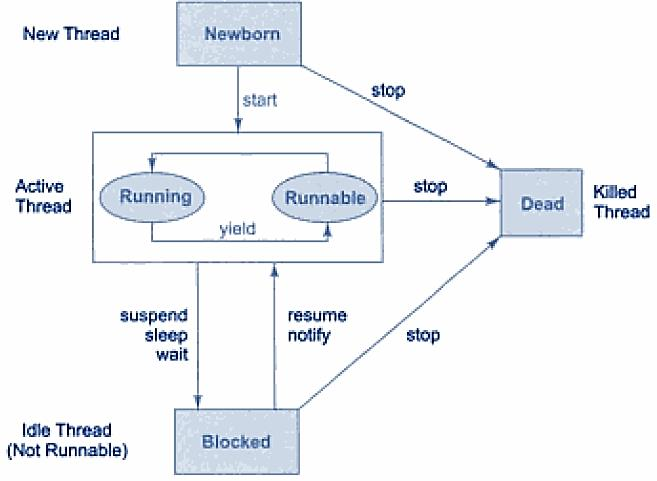
\includegraphics[scale=0.4]{ThreadStates.png}
\caption{Life cycle of a Thread}
\end{center}
\end{figure}


\begin{description}
\item [New] A thread that is just instantiated is in new state. When a \texttt{start()} method is invoked, the thread moves to the ready state from which it is automatically moved to runnable state by the thread scheduler. 
\item [Ready] The thread is in runnable state after invocation of \texttt{start()} method, but the thread scheduler has not selected it to be the running thread. 
\item [Running] The thread is in running state if the thread scheduler has selected it i.e, whenever the thread is under execution it is known as running state.
\item [Suspended] This is the state when the thread is still alive, but is currently not to executing. 
\item [Dead] A runnable thread enters the dead or terminated state when it completes its task or terminates. 
\end{description}

\section*{Thread Creation}
Java defines two ways in which this can be accomplished:
\begin{enumerate}
\item \textbf{Extending the \emph{Thread} Class}

The first way to create a thread is to create a new class that extends \texttt{Thread}, and then to create an instance of that class.
The extending class must override the \texttt{run()} method, which is the entry point for the new thread. It must also call \texttt{start()} to begin execution of the new thread.


\begin{figure}[ht]
\begin{center}
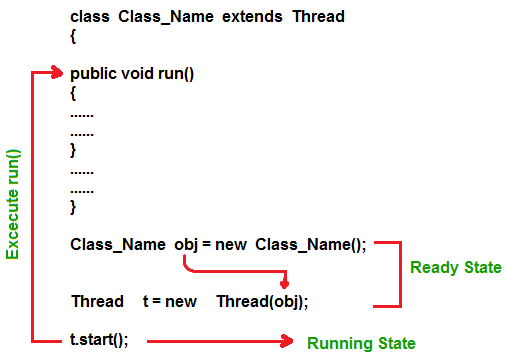
\includegraphics[scale=0.6]{Extends-Thread-Class.png}
\caption{creating thread by extending \texttt{Thread} class}
\end{center}
\end{figure}

 


Here, when extending the \texttt{Thread} class, the derived class cannot extend any other base classes because Java only allows single inheritance. 

This means that this class cannot inherit from any other class. Another way to program threads is by implementing \texttt{Runnable} interface.

\item \textbf{Implementing the Runnable Interface}
This is useful approach to create a thread because we can implement
The steps for creating a thread by using this mechanism are:
\begin{description} %[leftmargin=1.6cm]
\item[Step 1] Create a class that implements the interface \texttt{Runnable} and override \texttt{run()} method.

\begin{lstlisting}[numbers=none]
class MyThread implements Runnable {
    public void run() {
        // thread body of execution
    }
}
\end{lstlisting}

\item[Step 2] Creating Object
\begin{lstlisting}[numbers=none]
MyThread myObject = new MyThread();
\end{lstlisting}
\item[Step 3] Creating \texttt{Thread} object
\begin{lstlisting}[numbers=none]
Thread thread = new Thread(myObject);
\end{lstlisting}
\item[Step 4] Start execution of a thread
\begin{lstlisting}[numbers=none]
thread.start();
\end{lstlisting}
\end{description}

An example program illustrating creation and invocation of a thread object is given below:

\lstinputlisting{../Code/MyThreadRunnable.java}
In the above program, we created an object to MyThreadRunnable class. This object contains only run() but we need start() to initiate the thread thus, we attached this object to Thread object(thread).
\end{enumerate}
\subsection*{Thread Class Methods}
\begin{description}
\item [sleep()] method causes the current thread to sleep for a specified amount of time in milliseconds.
\begin{verbatim}
    public static void sleep(long millis) throws 
        InterruptedException
\end{verbatim}
For example, the code below puts the thread in sleep state for 3 minutes.
\begin{lstlisting}[numbers=none]
try {
    Thread.sleep(3 * 60 * 1000); // thread sleeps for 3 minutes
} catch(InterruptedException ex) {}
\end{lstlisting}
\item [yield()] method pauses the currently executing thread temporarily for giving a chance to the remaining waiting threads of the same priority to execute. If there is no waiting thread or all the waiting threads have a lower priority then the same thread will continue its execution.
\begin{verbatim}
    public static void yield()
\end{verbatim}
\item [isAlive()] method returns \lstinline{true} if the thread upon which it is called has been started but not moved to the dead state.
\begin{verbatim}
    public final boolean isAlive()
\end{verbatim}
\item [join()] When a thread calls \texttt{join()} on another thread instance, the caller thread will wait till the called thread finishes execution.
\begin{verbatim}
    final void join() throws InterruptedException
\end{verbatim}
\texttt{join()} can also be specified with some timeout, in which case the thread waits at most milliseconds for this thread to die. If timeout specified as `0' means the thread will wait forever.
\begin{verbatim}
    final void join(long millis) throws InterruptedException
    final void join(long millis, int nanos) throws 
        InterruptedException
\end{verbatim}
A thread waiting because of \texttt{join()} can also be interrupted. Hence the method throws a \texttt{InterruptedException}.
\end{description}

\subsection*{Naming Threads}
Every thread is given a name. If you don't specify a name, a default name will be created. For example the main thread is named ``main''.
The default name of a user defined thread is ``Thread-0'' for the first thread created, ``Thread-1'' for the second and so on. 
The Thread class provides methods to change and get the name of a thread. 
\begin{description}
\item [public void setName(String name)] is used to change the name of a thread.
\item [publie String getName()] returns the name of a thread.
\end{description}

\subsection*{Thread Priority}
Every Java thread has a priority that helps the operating system determine the order in which threads are scheduled.

Java priorities are in the range between \texttt{MIN\_PRIORITY (a constant of 1)} and \texttt{MAX\_PRIORITY (a constant of 10)}. By default, every thread is given priority \texttt{NORM\_PRIORITY (a constant of 5)}.

Threads with higher priority are more important to a program and should be allocated processor time before lower-priority threads. However, thread priorities cannot guarantee the order in which threads execute and very much platform dependent.
\lstinputlisting{../Code/NameAndPriority.java}

\subsection*{Daemon Threads}
So far the threads that have been created are called foreground threads. A program continues to execute as long as it has at least one
foreground (non-daemon) thread that is alive. The daemon threads are also called service threads. They are used for background processes that will continue only as long as the active threads of the program are alive.

Daemon threads cease to execute when there are no non-daemon threads alive because when VM detects that the only remaining threads are daemon threads, it exits. 



\emph{Note: garbage collector thread is a daemon thread that runs with a low priority.}
\subsection*{Example}
\lstinputlisting{../Code/DollDaemon.java}

\section*{Synchronization}
Whenever multiple threads are trying to use same resource then their may be a chance of getting wrong output, to overcome this problem thread synchronization can be used.

Allowing only one thread at a time to utilize the same resource out of multiple threads is known as thread synchronization or thread safe.

Java implements this concept by using \texttt{synchronized} keyword. \texttt{synchronized} can be used in 2 ways.
\begin{enumerate}
\item A method can be marked \texttt{synchronized}
\item A block of code can be marked \texttt{synchronized}
\end{enumerate}
\subsection*{Why threads synchronization?}
\begin{itemize}
\item Let us say we have an Account class which has withdraw and deposit methods.
\item For each transaction (deposit or withdraw) a thread is created.
\item Let us visualize what happens when two people simultaneously withdraw from the same account object .
\item Let us assume that there is Rs. 1000 in the account.
\end{itemize}

\begin{figure}[ht]
\begin{center}
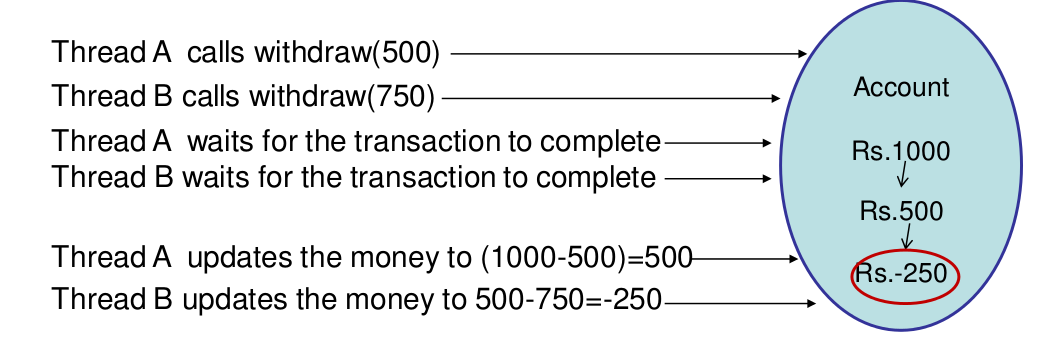
\includegraphics[scale=0.26]{WhySynchronization.png}
\end{center}
\end{figure}

\subsection*{Example - Code without synchronization}
\lstinputlisting{../Code/AccountUpdate.java}

%\vspace{\fill}
%\pagebreak

\subsection*{Solution to the Account problem}
\begin{figure}[ht]
\begin{center}
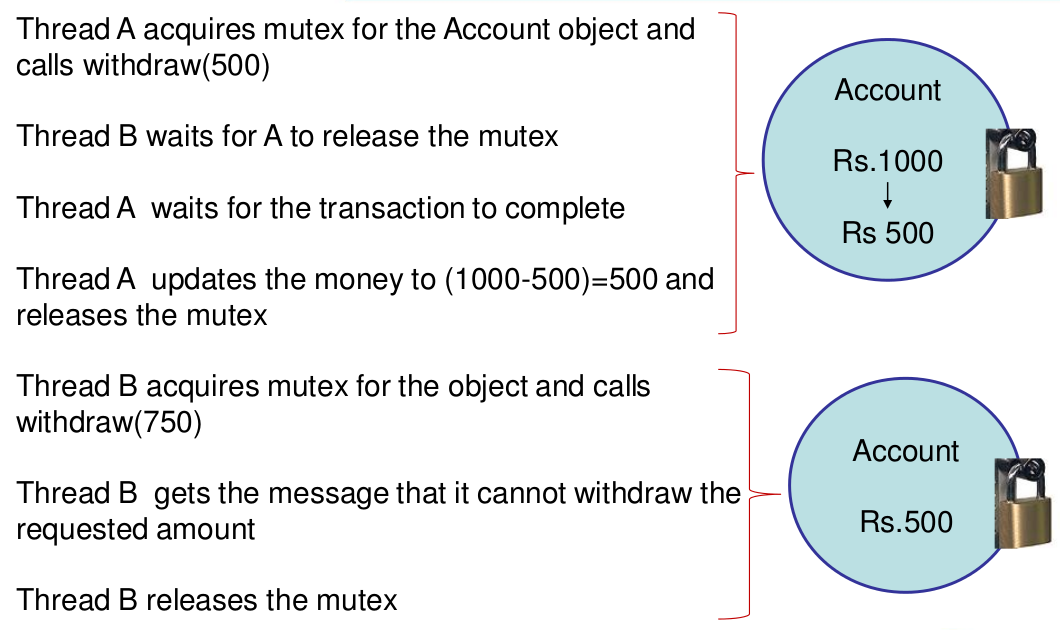
\includegraphics[scale=0.26]{SolutionSynchronized.png}
\end{center}
\end{figure}
\subsection*{Example - Code using synchronization}
If an object is visible to more than one thread, all reads or writes to that object's non final attributes should be done through
\texttt{synchronized} methods.
\begin{description}
\item [Approach 1:]  Add \texttt{synchronized} keyword to withdraw and other critical methods of the \texttt{Account} object.
\begin{verbatim}
synchronized void withdraw(int amt)
\end{verbatim}
\item [Approach 2:] Use \texttt{synchronized} statements by explicitly locking the object before calling critical methods of the \texttt{Account} object. 
\begin{verbatim}
public void run() {
    synchronized(a) {
        a.withdraw(amt); 
    }
}
\end{verbatim}
\end{description}

\section*{Inter-Thread Communication}
Inter-thread communication is required when execution of one thread depends on another thread's task. In such case, the second thread intimates or notifies the first thread when it has finished some task that the first thread is waiting for. The best suited situation to understand this is a producer-consumer problem.

A producer thread produces something which consumer thread consumes. A producer and consumer thread can run independently. Producer makes sure that it has produced enough for consumer to consume. If producer has not produced then consumer will have to wait till producer finishes.
\lstinputlisting{../Code/ProducerConsumerThreads.java}

\end{document}

